\documentclass[journal,12pt,twocolumn]{IEEEtran}
\usepackage{setspace}
\usepackage{gensymb}
\singlespacing
\usepackage[cmex10]{amsmath}
\usepackage{amsthm}
\usepackage{tcolorbox}
\usepackage{mathrsfs}
\usepackage{txfonts}
\usepackage{stfloats}
\usepackage{bm}
\usepackage{cite}
\usepackage{cases}
\usepackage{subfig}
\usepackage{tasks}
\usepackage{longtable}
\usepackage{multirow}
\usepackage{enumerate}
\usepackage{mathtools}
\usepackage{steinmetz}
\usepackage{tikz}
\usepackage{circuitikz}
\usepackage{verbatim}
\usepackage{tfrupee}
\usepackage[breaklinks=true]{hyperref}
\usepackage{graphicx}
\usepackage{tkz-euclide}
\usetikzlibrary{calc,math}
\usepackage{listings}
    \usepackage{color}                                            %%
    \usepackage{array}                                            %%
    \usepackage{longtable}                                        %%
    \usepackage{calc}                                             %%
    \usepackage{multirow}                                         %%
    \usepackage{hhline}                                           %%
    \usepackage{ifthen}                                           %%
    \usepackage{lscape}     
\usepackage{multicol}
\usepackage{chngcntr}

\DeclareMathOperator*{\Res}{Res}

\renewcommand\thesection{\arabic{section}}
\renewcommand\thesubsection{\thesection.\arabic{subsection}}
\renewcommand\thesubsubsection{\thesubsection.\arabic{subsubsection}}

\renewcommand\thesectiondis{\arabic{section}}
\renewcommand\thesubsectiondis{\thesectiondis.\arabic{subsection}}
\renewcommand\thesubsubsectiondis{\thesubsectiondis.\arabic{sub subsection}}


\hyphenation{optical networks semiconduc-tor}
\def\inputGnumericTable{}                                 %%

\lstset{
%language=C,
frame=single, 
breaklines=true,
columns=fullflexible
}
\begin{document}
\newcommand{\BEQA}{\begin{eqnarray}}
\newcommand{\EEQA}{\end{eqnarray}}
\newcommand{\define}{\stackrel{\triangle}{=}}
\bibliographystyle{IEEEtran}
\raggedbottom
\setlength{\parindent}{0pt}
\providecommand{\mbf}{\mathbf}
\providecommand{\pr}[1]{\ensuremath{\Pr\left(#1\right)}}
\providecommand{\qfunc}[1]{\ensuremath{Q\left(#1\right)}}
\providecommand{\fn}[1]{\ensuremath{f\left(#1\right)}}
\providecommand{\e}[1]{\ensuremath{E\left(#1\right)}}
\providecommand{\sbrak}[1]{\ensuremath{{}\left[#1\right]}}
\providecommand{\lsbrak}[1]{\ensuremath{{}\left[#1\right.}}
\providecommand{\rsbrak}[1]{\ensuremath{{}\left.#1\right]}}
\providecommand{\brak}[1]{\ensuremath{\left(#1\right)}}
\providecommand{\lbrak}[1]{\ensuremath{\left(#1\right.}}
\providecommand{\rbrak}[1]{\ensuremath{\left.#1\right)}}
\providecommand{\cbrak}[1]{\ensuremath{\left\{#1\right\}}}
\providecommand{\lcbrak}[1]{\ensuremath{\left\{#1\right.}}
\providecommand{\rcbrak}[1]{\ensuremath{\left.#1\right\}}}
\theoremstyle{remark}
\newtheorem{rem}{Remark}
\newcommand{\sgn}{\mathop{\mathrm{sgn}}}
\providecommand{\abs}[1]{\vert#1\vert}
\providecommand{\res}[1]{\Res\displaylimits_{#1}} 
\providecommand{\norm}[1]{\lVert#1\rVert}
\providecommand{\mtx}[1]{\mathbf{#1}}
\providecommand{\mean}[1]{E[ #1 ]}
\providecommand{\fourier}{\overset{\mathcal{F}}{ \rightleftharpoons}}
\providecommand{\system}{\overset{\mathcal{H}}{ \longleftrightarrow}}
\newcommand{\solution}{\noindent \textbf{Solution: }}
\newcommand{\cosec}{\,\text{cosec}\,}
\providecommand{\dec}[2]{\ensuremath{\overset{#1}{\underset{#2}{\gtrless}}}}
\newcommand{\myvec}[1]{\ensuremath{\begin{pmatrix}#1\end{pmatrix}}}
\newcommand{\mydet}[1]{\ensuremath{\begin{vmatrix}#1\end{vmatrix}}}
\numberwithin{equation}{subsection}
\makeatletter
\urlstyle{same}
\title{Assignment  }
\author{Harshal Verma\\
AI21MTECH02003}
\date{April 2021}
\maketitle
Download the source code and LaTex file from :
\begin{tcolorbox}
Code source: \url{https://github.com/harshal9876/AI5002/blob/main/Assignment_8/Codes/Assignemnt_8.py} \\
LaTex code :
\url{https://github.com/harshal9876/AI5002/blob/main/Assignment_8/Assignment_8.tex}
\end{tcolorbox}
\section{GATE 7}
Problem: Given Set A =  \{2,3,4,5\}  and Set B =
\{11,12,13,14,15\}, two numbers are randomly
selected,one from each set. What is probability
that the sum of the two numbers equals 16? \\
(a) 0.20\\
(b) 0.25\\
(c) 0.30\\
(d) 0.33
\section{Solution}
Given A = \{ 2,3,4,5 \} and Set B = \{ 11,12,13,14,15 \} . the possible combinations of selecting one number from each set is :\\
\\
\{ (2,11),(2,12),(2,13),(2,14),(2,15),(3,11),(3,12),(3,13),\\(3,14),(3,15),(4,11),(,4,12),(4,13),(4,14),(4,15),(5,11),\\(5,12),(5,13),(5,14),(5,15) \} 
\\
\\
Let X and Y be the random variable from each set A and B respectively, represented by . 
\\
\[
    X = 
\begin{cases}
    1,& \text{if X is a number in set A}  \\
    0,              & \text{otherwise}
\end{cases}
\]

similarly ,\\
\[
    Y = 
\begin{cases}
    1,& \text{if Y is a number in set B}  \\
    0,              & \text{otherwise}
\end{cases}
\]
Given a number is chosen from set A and set B respectively , X =1 and Y =1 . Let : \\
\begin{align}
K  &= Y + X\\
K  &= 
\begin{cases}
1,& \text{if X + Y = 16}  \\
0,              & \text{otherwise}
\end{cases}
\end{align}
\\
The samples that sums up to 16 are \\
= \{ (2,14),(3,13),(4,12),(5,11) \}\\
\smallskip
Cardinality of the favourable events is : 4\\
Cardinality of the sample space is : 20\\
\smallskip
\begin{align}
\text{probability} &= \frac{\text{Favourable sample space}}{\text{Total number of outcomes }}\\
\text{probability} &= \frac{4}{20}\\
\text{probability} &= 0.2
\end{align}
\\
The required probability of getting a sum of 16 when choosing two numbers in random is 0.2 \\
\smallskip

\begin{figure}[htp]
    \centering
    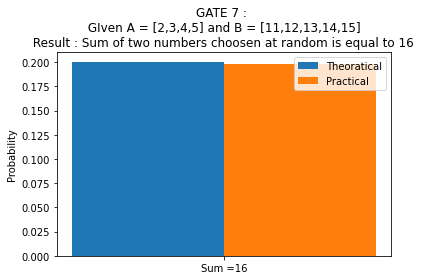
\includegraphics[width=10cm]{Assignemnt_8}
    \caption{Calculated versus theoretical probability}
    \label{fig :plot}
\end{figure}

\vfill
\end{document}



